\section{1174057 Alit Fajar Kurniawan}
\subsection{Teori}
	\subsubsection {Sejarah Perkembangan dan Definisi Artificial Intelligence}
	Kecerdasan buatan merupakan sebuah bidang dalam ilmu computer yang begitu penting di zaman ini dan masa yang akan datang guna mewujudkan sebuah sistem computer yang begitu cerdas. Artificial Intelligence atau biasa di singkat dengan AI berasal dari bahasa latin yang dimana intelligence berarti saya paham. 
	\par Pada tahun 1955, Newell dan juga Simon telah mengembangkan The Logic Theorist, yaitu program AI pertama. Dimana program tersebut mempresentasikan sebuah masalah sebagai model pohon, lalu diselesaikan dengaan cara memilih cabang yang akan mewujudkan kesimpulan terbenar dan tepat. Program AI tersebut berdampak sangat besar dan dapat mendaji batu loncatan yang cukup penting dalam mengembangkan bidang AI \cite{baraja2008kecerdasan}.
	\par
	Masa Perkembangan AI dimulai pada awal era komputer elektronik pada tahun 1941. dimana ditemukannya alat penyimpanan dan pemrosesan informasi. kemudian dilanjutkan pada masa-masa persiapan AI yang terjadi pada tahun 1943-1956. Pada sekitaran tahun 1952-1969 merupakan masa awal perkembangan AI terjadi, dan pada tahun 1966-1974 perkembangan AI mengalami penurunan atau melambatnya proses dalam melakukan pengembangan. pada tahun 1969 sampai 10 tahun kedepan kembali terjadi perkembangan yang menciptakan inovasi sistem berbasis pengetahuan. dan sekitaran tahun 1980-an AI kembali menjadi sebuah industri yang terus berkembang sampai sekarang ini.


	\subsubsection{learning, klasifikasi, regresi dan unsupervised learning. Data set, training set dan testing set}
	\begin{enumerate}
	\item
	Definisi Supervised Learning Dan Unsupervised Learning
	\subitem
	Supervised Learning merupakan suatu pendekatan yang dimana terdapat data dan variable yang telah ditargetkan sehingga pendekatan tersebut bertujuan untuk dapat mengelompokkan sebuah data ke data yang sudah ada, beda dengan Unsupervised learning yang tidak mempunyai data, sehingga data yang ada harus di kelompokkan menjadi beberapa bagian.
	\item
	Definisi  Klasifikasi Dan Regresi
	\subitem
	Klasifikasi adalah sebuah kegiatan penggolongan atau pengelompokkan. Menurut kamus besar bahasa Indonesia yang dimana klasifikasi merupakan penyusunan sistem di dalam kelompok atau golongan berdasarkan kaidah atau standar yang telah ditetapkan. Regresi adalah sebuah metode analisis statistic yang akan digunakan untuk melihat pengaruh variable.
	\item
	Devinisi Dataset, Training Set, Dan Testing Set
	\subitem
	Dataset adalah sebuah objek yang akan mempresentasikan sebuah data dan relasinya di memory. Struktur pada dataset ini mirip dengan data yang ada di dalam database. Training set adalah bagian dari dataset yang berperan dalam membuat prediksi atau algoritma sesuai tujuan masing–masing. Testing set adalah bagian dari dataset yang akan di tes guna melihat keakuratatan atau ketepatan datanya.
	\end{enumerate}

\subsection{Praktek}
	\subsubsection{Instalasi}
	\begin{enumerate}
		\item Melakukan instalasi library scikit pada anaconda, ketik kan pip install -U scikit-learn pada terminal anaconda. 

		\begin{figure}[H]
		\centering
		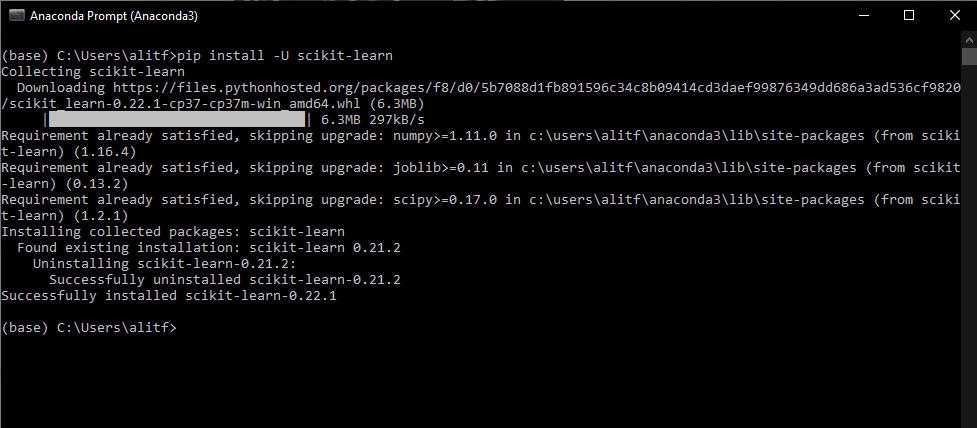
\includegraphics[width=1\textwidth]{figures/1174057/chapter1/1.png}
		\caption{Instalasi Scikit Learn}
		\label{print}
		\end{figure}

		\item Setelah selesai instalasi, pilih salah satu example dari website Scikit. 
		\begin{figure}[H]
		\centering
		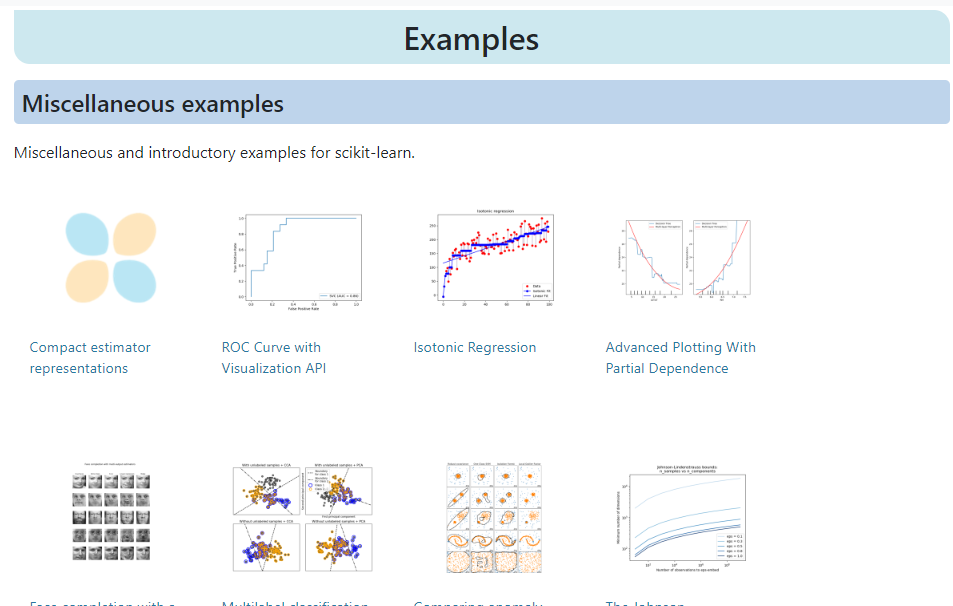
\includegraphics[width=1\textwidth]{figures/1174057/chapter1/2.png}
		\caption{Example}
		\label{print}
		\end{figure}

		\lstinputlisting[firstline=1, lastline=19]{src/1174057/chapter1/example.py}
		\par kemudian coba jalankan, lihat hasilnya
		\begin{figure}[H]
		\centering
		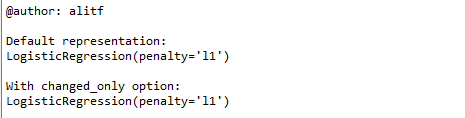
\includegraphics[width=1.5\textwidth]{figures/1174057/chapter1/3.png}
		\caption{Example}
		\label{print}
		\end{figure}

		\item latihan 2 Mencoba Loading an example dataset
		\lstinputlisting[firstline=1, lastline=9]{src/1174057/chapter1/dataset.py}
		\subitem hasil dari data digits
		\begin{figure}[H]
		\centering
		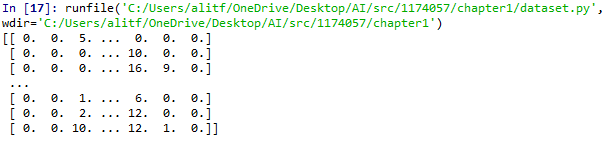
\includegraphics[width=1.5\textwidth]{figures/1174057/chapter1/4.png}
		\caption{Result Data Digits}
		\label{print}
		\end{figure}

		\subitem hasil dari digits.target
		\begin{figure}[H]
		\centering
		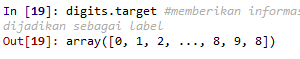
\includegraphics[width=1\textwidth]{figures/1174057/chapter1/5.png}
		\caption{Result digits.target}
		\label{print}
		\end{figure}

		\subitem hasil dari digits.image
		\begin{figure}[H]
		\centering
		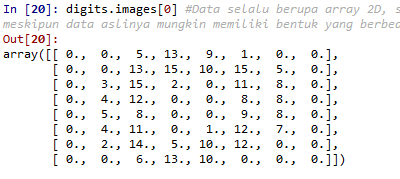
\includegraphics[width=1\textwidth]{figures/1174057/chapter1/6.png}
		\caption{Result digits.image}
		\label{print}
		\end{figure}

		\item latihan 3 Mencoba Learning and predicting
		\lstinputlisting[firstline=1, lastline=9]{src/1174057/chapter1/learning.py}
		\par kemudian coba jalankan, lihat hasilnya
		\begin{figure}[H]
		\centering
		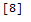
\includegraphics[width=1\textwidth]{figures/1174057/chapter1/7.png}
		\caption{Result Learning and predicting}
		\label{print}
		\end{figure}

		\item latihan 4 Mencoba Model persistence
		\lstinputlisting[firstline=1, lastline=16]{src/1174057/chapter1/modelpersistence.py}
		\par kemudian coba jalankan, lihat hasilnya
		\begin{figure}[H]
		\centering
		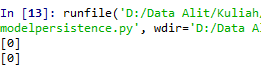
\includegraphics[width=1\textwidth]{figures/1174057/chapter1/8.png}
		\caption{Result Model persistence}
		\label{print}
		\end{figure}

		\item latihan 5 Mencoba Conventions
		\lstinputlisting[firstline=1, lastline=46]{src/1174057/chapter1/conventions.py}
		\par kemudian coba jalankan, lihat hasilnya
		\begin{figure}[H]
		\centering
		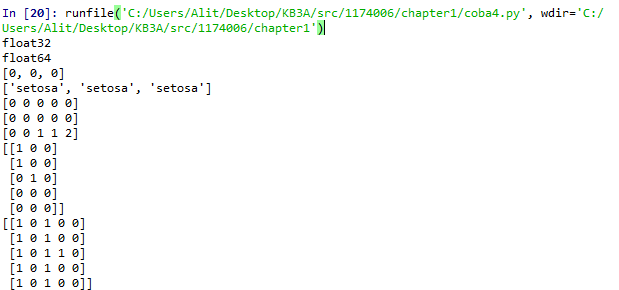
\includegraphics[width=1\textwidth]{figures/1174057/chapter1/9.png}
		\caption{Result Conventions}
		\label{print}
		\end{figure}

	\end{enumerate}

\subsection{Penanganan Error}
	\begin{enumerate}
		\item Screenshoot Error
		\begin{figure}[H]
		\centering
		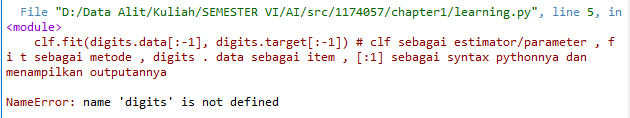
\includegraphics[width=1\textwidth]{figures/1174057/chapter1/error1.png}
		\caption{Error}
		\label{print}
		\end{figure}

		\begin{figure}[H]
		\centering
		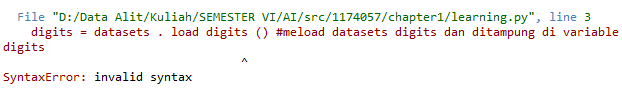
\includegraphics[width=1\textwidth]{figures/1174057/chapter1/error2.png}
		\caption{Error}
		\label{print}
		\end{figure}

		\item Tuliskan kode dan jenis error
			\subitem is not defined, xception yang terjadi saat syntax melakukan eksekusi terhadap local name atau global name yang tidak terdefinisi.
			\subitem invalid syntax

		\item Solusi penanganan error
			\subitem Solusinya adalah memastikan variabel atau function yang dipanggil ada atau tidak salah ketik. 
			\subitem Periksa kembali syntax yang dibuat, bisa saja ada kesalahan dalam spasi.
	\end{enumerate}

\subsection{Bukti Tidak Plagiat}
	\begin{figure}[H]
		\centering
		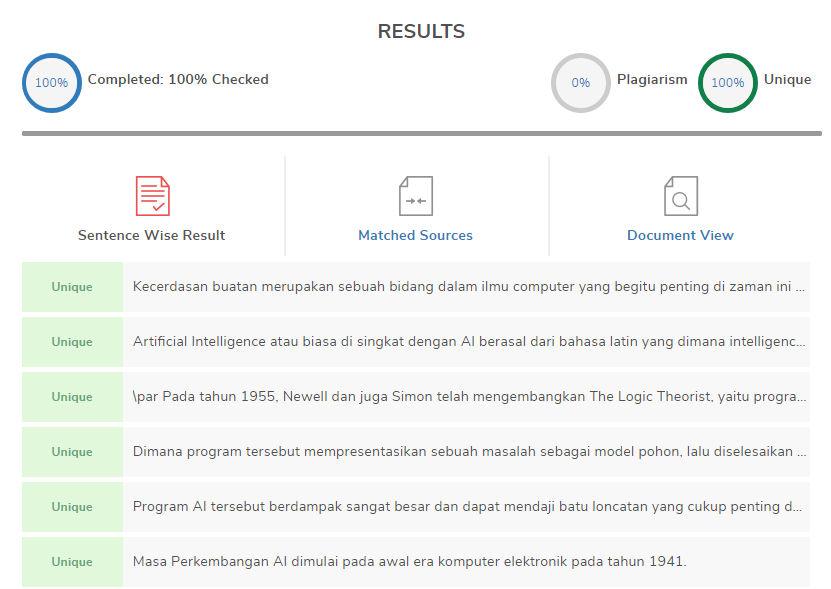
\includegraphics[width=1\textwidth]{figures/1174057/chapter1/plagiat.png}
		\caption{Plagiarisme}
		\label{print}
	\end{figure}